% Copyright (c)  2005-2010 EDF-EADS-PHIMECA.
% Permission is granted to copy, distribute and/or modify this document
% under the terms of the GNU Free Documentation License, Version 1.2
% or any later version published by the Free Software Foundation;
% with no Invariant Sections, no Front-Cover Texts, and no Back-Cover
% Texts.  A copy of the license is included in the section entitled "GNU
% Free Documentation License".
\renewcommand{\filename}{docUC_CentralUncertainty_TaylorVarDecomposition.tex}
\renewcommand{\filetitle}{UC : Moments evaluation from the Taylor variance decomposition method and evaluation of the importance factors associated}

% \HeaderNNIILevel
% \HeaderIILevel
\HeaderIIILevel


\index{Taylor variance decomposition }
\index{Graph!Taylor variance decomposition  importance factors}
\index{Graph Manipulation!ViewImage}
\index{Graph Manipulation!Show}

The objective of this Use Case  is to evaluate the mean and standard deviation of the output variable of interest thanks to the Taylor variance decomposition method of order one or two.\\

Details on the  Taylor variance decomposition method may be found in the Reference Guide (\href{OpenTURNS_ReferenceGuide.pdf}{see files Reference Guide - Step C -- Taylor variance decomposition / Perturbation Method} and Step C' -- importance Factors derived from Taylor Variance Decomposition Method).\\

Details on each object may be found in the User Manual  (\href{OpenTURNS_UserManual_TUI.pdf}{see User Manual - Taylor variance decomposition of the limit state function / QuadraticCumul}).\\




\requirements{
  \begin{description}
  \item[$\bullet$] None
  \end{description}
}
{
  \begin{description}
  \item[$\bullet$] Mean and covariance of the variable of interest
  \item[type:] NumericalPoint, Matrix
  \item[$\bullet$] Importance factors from the Taylor variance decomposition method only for {\itshape output} of dimension 1
  \item[type:] NumericalPoint
  \end{description}
}

\textspace\\
Python script for this UseCase :
T
\begin{lstlisting}

  # To have a beautifull graph of importance factors,
  # give the output random variable a name
  output.setName("Output_1")

  # Create a quadraticCumul algorithm
  myQuadraticCumul = QuadraticCumul(output)

  # Stream out the result
  print "myQuadraticCumul=", myQuadraticCumul

  # Compute the several elements provided by the quadratic cumul algorithm
  # First order mean
  print "First order mean=", myQuadraticCumul.getMeanFirstOrder()
  # Second order mean
  print "Second order mean=", myQuadraticCumul.getMeanSecondOrder()
  # Covariance Matrix
  print "Covariance=", myQuadraticCumul.getCovariance()
  # Importance factors
  # CARE : for this calculus only, the output variable of interest must be of dimension 1
  print "Importance factors=", myQuadraticCumul.getImportanceFactors()

  # Graph 1 : Importance Factors graph
  importanceFactorsGraph = myQuadraticCumul.drawImportanceFactors()

  # In order to see the graph without creating the associated files
  Show(importanceFactorsGraph)

  # Create the .PNG, .EPS and .FIG files
  importanceFactorsGraph.draw("ImportanceFactorsDrawingQuadraticCumul")

  # View the bitmap file
  ViewImage(importanceFactorsGraph.getBitmap())

  # Check if it worked
  print "bitmap=" , importanceFactorsGraph.getBitmap()
  print "postscript=", importanceFactorsGraph.getPostscript()

  # Get the  value of the limit state function at the mean point
  meanValue = getValueAtMean()

  # Get the gradient value of the limit state function at the mean point
  meanGrandient = getGradientAtMean()

  # Get the hessian value of the limit state function at the mean point
  meanHessian = getHessianAtMean()
\end{lstlisting}
\textspace\\




Figure \ref{quadraticCumulImportanceFactors}  shows an importance factors pie evaluated from the Taylor variance decomposition method, in the beam example described in Eq.(\ref{equatPoutre}) before, where :
\begin{itemize}
\item $E$ follows the Beta($r = 0.94$, $t = 3.19$, $a = 2.78e7$, $b = 4.83e7$) distribution,
\item $F$ follows the LogNormal($\mu = 3e5$, $\sigma = 9e3$, $\gamma = 1.5e4$)  distribution,
\item $L$ follows the Uniform($a = 250$, $b=260$) distribution,
\item $I$ follows the Beta($r = 2.5$, $t = 4.0$, $a = 3.1e2$, $b = 4.5e2$) distribution,
\item the four components are independent.
\end{itemize}



\begin{figure}[H]
  \begin{center}
    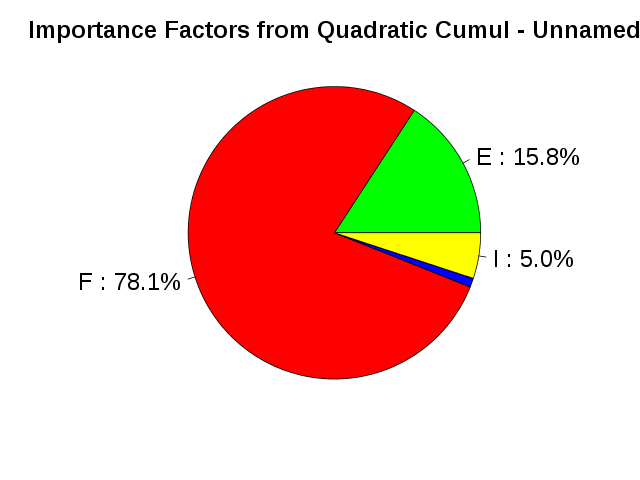
\includegraphics[width=10cm]{ImportanceFactorsDrawingQuadraticCumul.png}
  \end{center}
  \caption{Importance Factors from the Taylor variance decomposition method in the beam example.}
  \label{quadraticCumulImportanceFactors}
\end{figure}



